\chapter{Testy aplikacji}
\section{Testy jednostkowe}
	Przeprowadzone testy jednostkowe sprawdzały poprawność logiki programu.
	Testowaną warstwą jest więc warstwa \emph{Core}.
	Podczas testów wykorzystano bibliotekę \emph{xunit}.
	Listing~\ref{lst:unitTest} przedstawia test sprawdzający poprawność dodawania oceny albumu.
	Po dodaniu oceny aktualizowana jest średnia ocena.
	Test przeprowadzono dla wartości zwracającej liczbę zmiennoprzecinkową, aby upewnić się że dzielenie wykonywane jest prawidłowo.
	Jako wartość początkową ustawiono album z dwoma ocenami dającymi średnią równą 2.
	Następnie dodano ocenę o wartości 4 i sprawdzono, czy nowa średnia jest równa 8/3.

	\begin{lstlisting}[label=lst:unitTest, caption=Test jednostkowy dodawania oceny albumu, float=h]
		[Fact]
		public void AddSubsequentRating()
		{
			var ratings = new List<Rating>
			{
				new RatingBuilder().WithDefaultValues()
				.Stars(1).Build(),
				new RatingBuilder().WithDefaultValues()
				.Stars(3).Build()
			};

			var album = new AlbumBuilder().WithDefaultValues()
				.Ratings(ratings).Build();

			var newRating = new RatingBuilder().WithDefaultValues()
				.Stars(4).Build();

			album.AddRating(newRating);

			var expected = (float)(8.0 / 3);
			Assert.Equal(expected, album.AverageRating);
		}
	\end{lstlisting}

\section{Testy integracyjne}
	Testy integracyjne sprawdzają zgodność komunikacji pomiędzy komponentami.
	Przeprowadzone zostały testy wykorzystujące wszystkie trzy warstwy serwisu API.
	Aby było to możliwe, zaimplementowano serwer testowy przy pomocy biblioteki \emph{AspNetCore.Mvc.Testing} (Listing~\ref{lst:testServer}).
	Klasa \verb|WebApplicationFactory| pozwala na stworzenie serwera, który obsługuje zapytania HTTP,
	bezpośrednio w pamięci podczas wykonywania testów.
	W serwerze skonfigurowano jedynie podstawowe wymagane serwisy:
	\begin{itemize}
		\item GraphQL wykorzystujące te same typy, co serwis API,
		\item AppDbContext łączące się do bazy w pamięci
		\item IRepository i jego implementację z warstwy \emph{Infrastructure}
	\end{itemize}
	Na sam koniec wywołano funkcję \verb|SeedData.PopulateTestData|, dodającą dane testowe do bazy.

	Na listingu~\ref{lst:integrationTest} przedstawiono test wykorzystujący tą klasę.
	Sprawdzane jest, czy oprócz wczytywania i formatowania danych z bazy, poprawnie odbywa się ładowanie pokrewnych wpisów (\verb|albumArtist|).
	Na początku definiowane jest zapytanie w języku GraphQL, które
	zwraca tytuł albumu oraz nazwę wykonwacy.
	Dane te są porównywane ze znanymi, domyśnymi danymi w bazie.


	\begin{lstlisting}[label=lst:testServer, caption=Serwer do testów, float=h]
		public class WebAppTestFactory<TStartup> : WebApplicationFactory<Startup>
		{
			protected override void ConfigureWebHost(IWebHostBuilder builder)
			{
				builder
					.Configure(app => app.UseGraphQL("/"))
					.ConfigureServices(services =>
				{
					var serviceProvider = new ServiceCollection()
						.AddEntityFrameworkInMemoryDatabase()
						.AddEntityFrameworkProxies()
						.BuildServiceProvider();
	
					services.AddDbContext<AppDbContext>(options =>
					{
						options.UseInMemoryDatabase("TestDB");
						options.UseLazyLoadingProxies();
						options.UseInternalServiceProvider(serviceProvider);
					});
					services.AddScoped<IRepository, EfRepository>();
	
					services.AddGraphQL(sp => SchemaBuilder.New()
						.AddServices(sp)
						.AddQueryType<QueryType>()
						.AddMutationType<MutationType>()
						.BindClrType<Guid, IdType>()
						.Create());
	
					var sp = services.BuildServiceProvider();
	
					using (var scope = sp.CreateScope())
					{
						var scopedServices = scope.ServiceProvider;
						var db = scopedServices.GetRequiredService<AppDbContext>();
	
						db.Database.EnsureCreated();
						SeedData.PopulateTestData(db);
					}
				});
			}
		}
	\end{lstlisting}

	\begin{lstlisting}[label=lst:integrationTest, caption=Test integracyjny zapytania GraphQL, float]
		public class GraphQLTests : IClassFixture<WebAppTestFactory<Startup>>
		{
			private readonly HttpClient _client;

			public GraphQLTests(WebAppTestFactory<Startup> factory)
			{
				_client = factory.CreateClient();
			}

			[Fact]
			public async Task ReturnsAlbumWithArtist()
			{
				var request = new JObject();
				request.Add("query",
					"query getAlbum{ album(id: \"b0000000000000000000000000000001\")" +
					"{ title albumArtist {name}}}");

				var response = await _client.PostAsync("/", new StringContent(
					request.ToString(), Encoding.UTF8, "application/json"));

				response.EnsureSuccessStatusCode();

				var responseString = await response.Content.ReadAsStringAsync();
				dynamic actual = JObject.Parse(responseString);

				Assert.Equal("Album 1", Convert.ToString(actual.data.album.title));
				Assert.Equal("Artist 1",
					Convert.ToString(actual.data.album.albumArtist.name));
			}
		}
	\end{lstlisting}

\section{Testy akceptacyjne}
	Przeprowadzone zostały testy akceptacyjne sprawdzające poprawność działania aplikacji.
	Aby przetestować API wykorzystano narzędzie \emph{Playground} przedstawione na zrzucie ekranu~\ref{fig:playground}.
	Pozwala ono na pisanie zapytań w języku GraphQL i wywoływać je na serwerze API.
	Dodatkowo, wczytuje schemat API dzięki czemu oferuje podpowiedzi podczas pisania zapytań.
	\begin{figure}[ht]
		\centering
			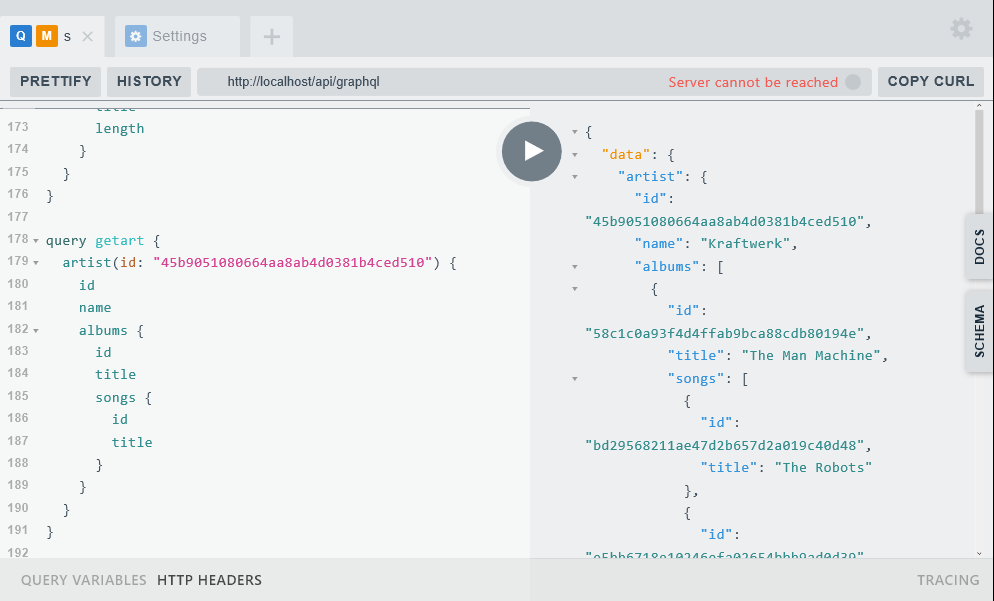
\includegraphics[width=\linewidth]{rys06/playground.png}
		 \caption{Narzędzie do testowania API GraphQL}
		 \label{fig:playground}
	\end{figure}

	Przeprowadzono również testy akceptacyjne procesu rejestracji i logowania użytkownika.
	Podczas tych testów upewniono się, że w konsoli przeglądarki nie można podejrzeć danych pozwalających na oszukanie systemu.
	Komunikacja była poprawnie zabezpieczona i zgodna z protokołem OpenID Connect z kodem autoryzacji i PKCE.

	W głównym interfejsie sprawdzono poprawność dodawania ocen i recenzji albumów.
	Albumy są poprawnie zwracane z API Last.fm, zarówno wyszukując po nazwie albumu, jak i po artyście.
	Po wybraniu albumu można poprawnie dodać do niego ocenę, a album zostanie wyświetlony na głównej liście.
